%!TEX root = ../report.tex

% 
% Objectives
% 

\section{Research Methodology}

To conduct this research we will use the Design Science Research Methodology (DSRM) \cite{DSRM} for presenting and validating a solution for this project's problem. As stated in \cite{DSRM}, \textit{``It involves a rigorous process to design artifacts to solve observed problems, to make research contributions, to evaluate the designs, and to communicate the results to appropriate audiences. Such artifacts may include constructs, models, methods, and instantiations"}. The artifacts can be constructs (vocabulary and symbols), models (abstractions and representations), methods (algorithms and practices) and instantiations (implemented and prototype systems). In this project we will focus on models and methods.\par
This methodology is based in seven guidelines that describe well conducted researches: it most produce an artifact created to address a problem, the artifact must be relevant to the solution, its utility, quality and efficacy must be rigorously evaluated, the research should present a verifiable contribution, rigor must be applied in development and evaluation, development should be based in existing knowledge and, finally, the research should be effectively communicated to appropriate audiences.\par
Information Systems can take several advantages from the use of DSRM as a research methodology because it is an knowledge area were theory from other areas are applied to solve problems at the intersection of IT and organizations.\cite{DSRM}
This methodology has three main objectives: provide a nominal process for the conduct of design science research, build upon prior literature about design science in Information Systems and reference disciplines and provide researchers with a mental model or template for a structure for research outputs. It consists in a iterative process composed by six phases:

\begin{itemize}
  \item \textbf{Problem identification and Motivation} - Definition of problem's importance and the necessity of a solution-
  \item \textbf{Define objectives of a solution} - Presentation of requirements that should be fulfilled by the solution to implement. 
  \item \textbf{Design and Development} - Key element of the DSR methodology where artifacts will be implemented to address requirements. This phase is iterative in the way it needs revisions and adjustments. It will receive feedback from ahead phases.
  \item \textbf{Demonstration} -  Confirmation of application of artifact to the problem's requirements.
  \item \textbf{Evaluation} - Measurement of the level in which the artifacts produced fulfill the initial problem.
  \item \textbf{Communication} - Documentation and spreading of the artifacts as the problem's solution.
\end{itemize}

\begin{figure}[h!]
\centering
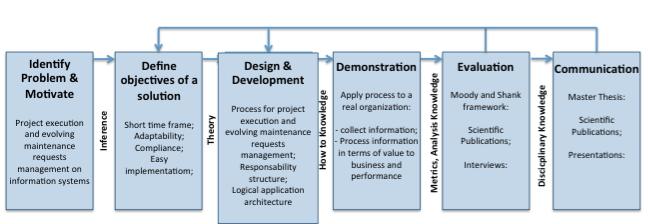
\includegraphics[width=\textwidth]{img/DSRMProcessMapping.png}
\caption{Project Mapping to DSRM Process}
\end{figure}


In Figure 1 we present the mapping between the DSRM process and this project research methodology. The next sections follow the methodology steps: Section 3 (Problem contextualization) will define problem context and its importance. In section 4 and 5 we present the state of the art in frameworks and standards for management and governance processes. In section 6 we present the state of the art for market solutions on ITSM and PPM tools. In section 7 we make a solution and demonstration proposal being section 8 reserved for the evaluation methodology.\par


